\documentclass[12pt,
	english,			% idioma adicional para hifenização
	french,				% idioma adicional para hifenização
	spanish,			% idioma adicional para hifenização
	brazil,				% o último idioma é o principal do documento
	]{article}

%% Language and font encodings
\usepackage[brazil]{babel}
\usepackage[utf8x]{inputenc}
\usepackage[T1]{fontenc}
\usepackage{indentfirst}
\usepackage{float}

%% Sets page size and margins
\usepackage[a4paper,top=3cm,bottom=2cm,left=3cm,right=3cm,marginparwidth=1.75cm]{geometry}

%% Useful packages
\usepackage{amsmath}
\usepackage{graphicx}
\usepackage[colorinlistoftodos]{todonotes}
\usepackage[colorlinks=true, allcolors=blue]{hyperref}
\usepackage{url}
\usepackage{listings}

\usepackage{xcolor}

\definecolor{codegreen}{rgb}{0,0.6,0}
\definecolor{codegray}{rgb}{0.5,0.5,0.5}
\definecolor{codepurple}{rgb}{0.58,0,0.82}
\definecolor{backcolour}{rgb}{0.95,0.95,0.92}

\lstdefinestyle{mystyle}{
    backgroundcolor=\color{backcolour},   
    commentstyle=\color{codegreen},
    keywordstyle=\color{magenta},
    numberstyle=\tiny\color{codegray},
    stringstyle=\color{codepurple},
    basicstyle=\ttfamily\footnotesize,
    breakatwhitespace=false,         
    breaklines=true,                 
    captionpos=b,                    
    keepspaces=true,                 
    numbers=left,                    
    numbersep=5pt,                  
    showspaces=false,                
    showstringspaces=false,
    showtabs=false,                  
    tabsize=2
}

\lstset{style=mystyle}

%% Document Header
\title{Laboratório 03 - CNN\\
\Large{Aprendizado de Máquina - INFO7004}\\
\Large{Prof. Luiz Eduardo S. Oliveira, Ph.D}}

\author{Discente: Marc Queiroz}
\date{08 de setembro de 2020}

%% Document Begin
\begin{document}
\maketitle

%\begin{abstract}

% Seu resumo do relatório, resumo não é introdução! Por exemplo, o excerto abaixo foi extraído do relatório de alunos do 1s2017, note que ele resume as atividades desenvolvidas e apresentadas no relatório, porém não faz uma introdução exagerada ao assunto abordado.
%"\textit{Calculamos a partir da montagem de circuitos RC e RLC a resistência interna do osciloscópio, bem como os valores de capacitância dos componentes utilizados. Analisamos as curvas dos circuitos passa-altas, passa-baixas e passa banda, juntamente com seus respectivos diagramas de bode, comparando-as com curvas esperadas fornecidas na literatura sobre o assunto. Utilizando um método baseado em assíndotas, estimamos valores para as frequências de ressonância e de corte, comparando-os com valores experimentais e teóricos}"

%\end{abstract}

\section{Introdução}

A prática do laboratório 3 apresenta um base de dados de imagens que apresentam escritas manuais com os meses do ano. A tarefa consiste em analisar a implementação e treinamento de CNNs e também a geração de imagens utilizando a técnica de \it{data augmentation}.

Este trabalho investiga os impactos da base de treinamento para 5 classificadores lineares:

\begin{itemize}
    \item kNN
    \item Naive Bayes
    \item Linear Discriminant Analysis
    \item Logistic Regression
    \item Perceptron
\end{itemize}

Com uma base de treinamento de 20000 entradas e teste de 58646 entradas, separadas em 10 classes e 132 características.

Este trabalho tem como objetivo resolver 5 atividades propostas. As próximas seções vão apresentar as respostas para o trabalho proposto.

Os códigos, gráficos e resultados desse relatório encontram-se disponíveis no repositório do GitHub, e podem ser acessados através do link: \url{https://github.com/marc-queiroz/ml_impactos_aprendizagem}.

\section{Atividade - I}

\textbf{Atividade:} Compare o desempenho desses classificadores em função da disponibilidade de base de treinamento. Alimente os classificadores com blocos de 1000 exemplos e plote num gráfico o desempenho na base de testes. Analise em qual ponto o tamanho da base de treinamento deixa de ser relevante.

Após implementar os classificadores e executá-los com blocos de 1000 até 20000, com passos de 1000, chegou-se ao gráfico de desempenho da figura \ref{fig:grafico01}.

\begin{figure}[H]
\centering
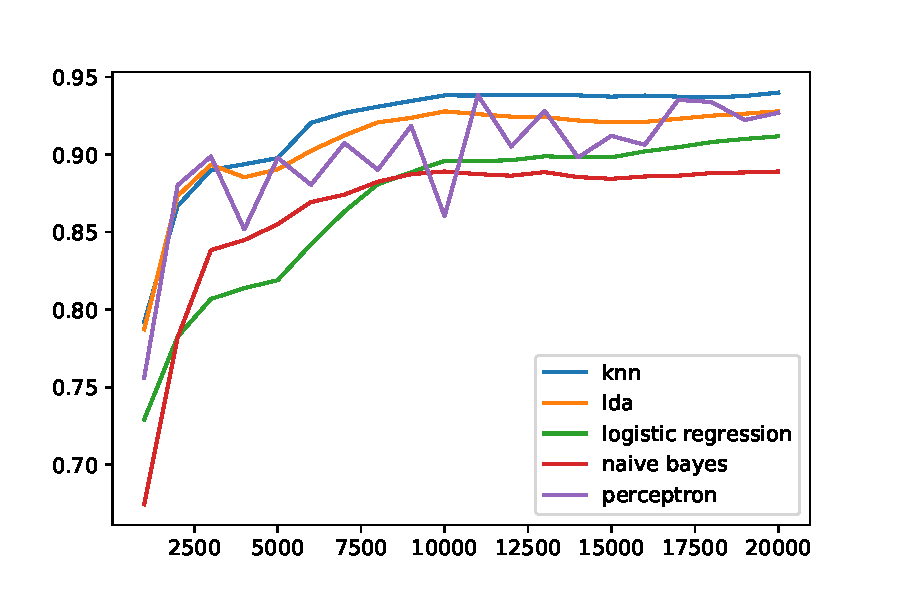
\includegraphics[width=1\textwidth]{grafico01.pdf}
\caption{\label{fig:grafico01}Gráfico de desempenho dos 5 classificadores}
\end{figure}

O tamanho da base de treinamento influencia cada classificador de maneira diferente, então alguns classificadores apresentaram resultados diferentes entre si. Apresentamos a tabela \ref{tab:tamanho} para enumerar cada um dos classificadores e o tamanho do bloco no qual a base de treinamento deixa de ser relevante.

\begin{table}[ht]
\centering
\begin{tabular}{|l|l|l|}
\hline
Classificador & \begin{tabular}[c]{@{}l@{}}Tamanho do \\ bloco de treino\end{tabular} & Acurácia \\ \hline
kNN & 8000 & 0.93 \\ \hline
LDA & 8000 & 0.92 \\ \hline
Logistic Regression & 19000 & 0.91 \\ \hline
Naive Bayes & 8000 & 0.88 \\ \hline
Perceptron & 9000 & 0.91 \\ \hline
\end{tabular}
\caption{\label{tab:tamanho}Tamanho da base de treinamento e acurácia máxima atingida}
\end{table}

Depois de verificar os resultados é possível perceber que os classificadores kNN, LDA e Naive Bayes estabilizam seu resultado com base de treinamento com tamanho de 8000. O Perceptron apresenta um resultado serrilhado, oscilando para diferentes tamanhos, mas apresenta um resultado satisfatório com 9000 entradas. Já o classificador, Logistic Regression precisou de 19000 entradas de treinamento para chegar ao seu resultado máximo.

\section{Atividade - II}

\textbf{Atividade:} Indique qual é o classificador que tem o melhor desempenho com poucos dados = 1000 exemplos. A tabela \ref{tab:tamanho1000} apresenta os resultados a serem analisados.

\begin{table}[H]
\centering
\begin{tabular}{|l|l|l|}
\hline
Classificador & \begin{tabular}[c]{@{}l@{}}Tamanho do \\ bloco de treino\end{tabular} & Acurácia \\ \hline
kNN & 1000 & 0.79 \\ \hline
LDA & 1000 & 0.78 \\ \hline
Logistic Regression & 1000 & 0.72 \\ \hline
Naive Bayes & 1000 & 0.67 \\ \hline
Perceptron & 1000 & 0.75 \\ \hline
\end{tabular}
\caption{\label{tab:tamanho1000}Tamanho da base = 1000 e acurácia comparada}
\end{table}

O kNN é o classificar com melhor desempenho para uma base de treinamento de 1000 entradas. Mas vale a pena ressaltar que o LDA também apresentou bom resultado.

\section{Atividade - III}\label{sec:3}

\textbf{Atividade:} Indique o classificador que tem melhor desempenho com todos os dados de treinamento. A tabela \ref{tab:tamanho20000} apresenta os resultados a serem analisados.

\begin{table}[ht]
\centering
\begin{tabular}{|l|l|l|}
\hline
Classificador & \begin{tabular}[c]{@{}l@{}}Tamanho do \\ bloco de treino\end{tabular} & Acurácia \\ \hline
kNN & 20000 & 0.94 \\ \hline
LDA & 20000 & 0.92 \\ \hline
Logistic Regression & 20000 & 0.91 \\ \hline
Naive Bayes & 20000 & 0.88 \\ \hline
Perceptron & 20000 & 0.75 \\ \hline
\end{tabular}
\caption{\label{tab:tamanho20000}Tamanho da base = 20000 e acurácia comparada}
\end{table}

O melhor desempenho é dado pelo classificar kNN atingindo uma acurácia de 94\% para uma base de treinamento de 20000 entradas.

\section{Atividade - IV}

\textbf{Atividade:} Indique o classificador mais rápido para classificar os 58k exemplos de teste.

Para responder essa atividade, o tempo de todos os testes foram capturados. Agrupando os classificadores e calculando o tempo médio para todos os testes realizados, pode-se apresentar a tabela \ref{tab:rapido}.

\begin{table}[H]
\centering
\begin{tabular}{|l|l|l|}
\hline
Classificador & \begin{tabular}[c]{@{}l@{}}Tamanho do \\ bloco de teste\end{tabular} & Tempo médio em (ms) \\ \hline
kNN & 58646 & 73.85 \\ \hline
LDA & 58646 & 0.02 \\ \hline
Logistic Regression & 58646 & 1.12 \\ \hline
Naive Bayes & 58646 & 0.56 \\ \hline
Perceptron & 58646 & 0.01 \\ \hline
\end{tabular}
\caption{\label{tab:rapido}Tamanho do teste 58646, comparada com o tempo médio de cada classificador}
\end{table}

O classificador mais rápido é o Perceptron com 0.01 ms de tempo médio, em segundo lugar o LDA com 0.02 ms.

\section{Atividade - V}

\textbf{Atividade:} Analise as matrizes de confusão. Os erros são os mesmos para todos os classificadores quando todos eles utilizam toda a base de treinamento?

Abaixo são apresentados as matrizes confusões para os 5 classificadores. As matrizes confusão apresentam a quantidade de acertos e erros por classe e também a sua porcentagem, que serão muito úteis para análise.

Como visto na seção \ref{sec:3}, \textbf{Atividade - III}, apontou-se que o melhor classificador é o kNN. Utilizando sua matriz confusão, figura \ref{fig:confusion_knn}, pode-se observar que a sua maior confusão foi entre as classes 3 e 5, com um erro de 6.8\% ou 377 erros.

Continuando com a análise, pode-se escolher o classificador LDA, que ficou em segundo lugar na \textbf{Atividade - III}. Utilizando sua matriz confusão, figura \ref{fig:confusion_lda}, pode-se observar que sua maior confusão foi entre as classe 8 e 9, com um erro de 6.3\% ou 361 erros.

É interessante observar que os dois classificadores, embora tenham acurácias parecidas, apresentem dificuldades em predizer classes diferentes.

Conclui-se que os erros não são os mesmos para todos os classificadores.

\begin{figure}[!htb]
  \begin{minipage}{.47\textwidth}
    \centering
    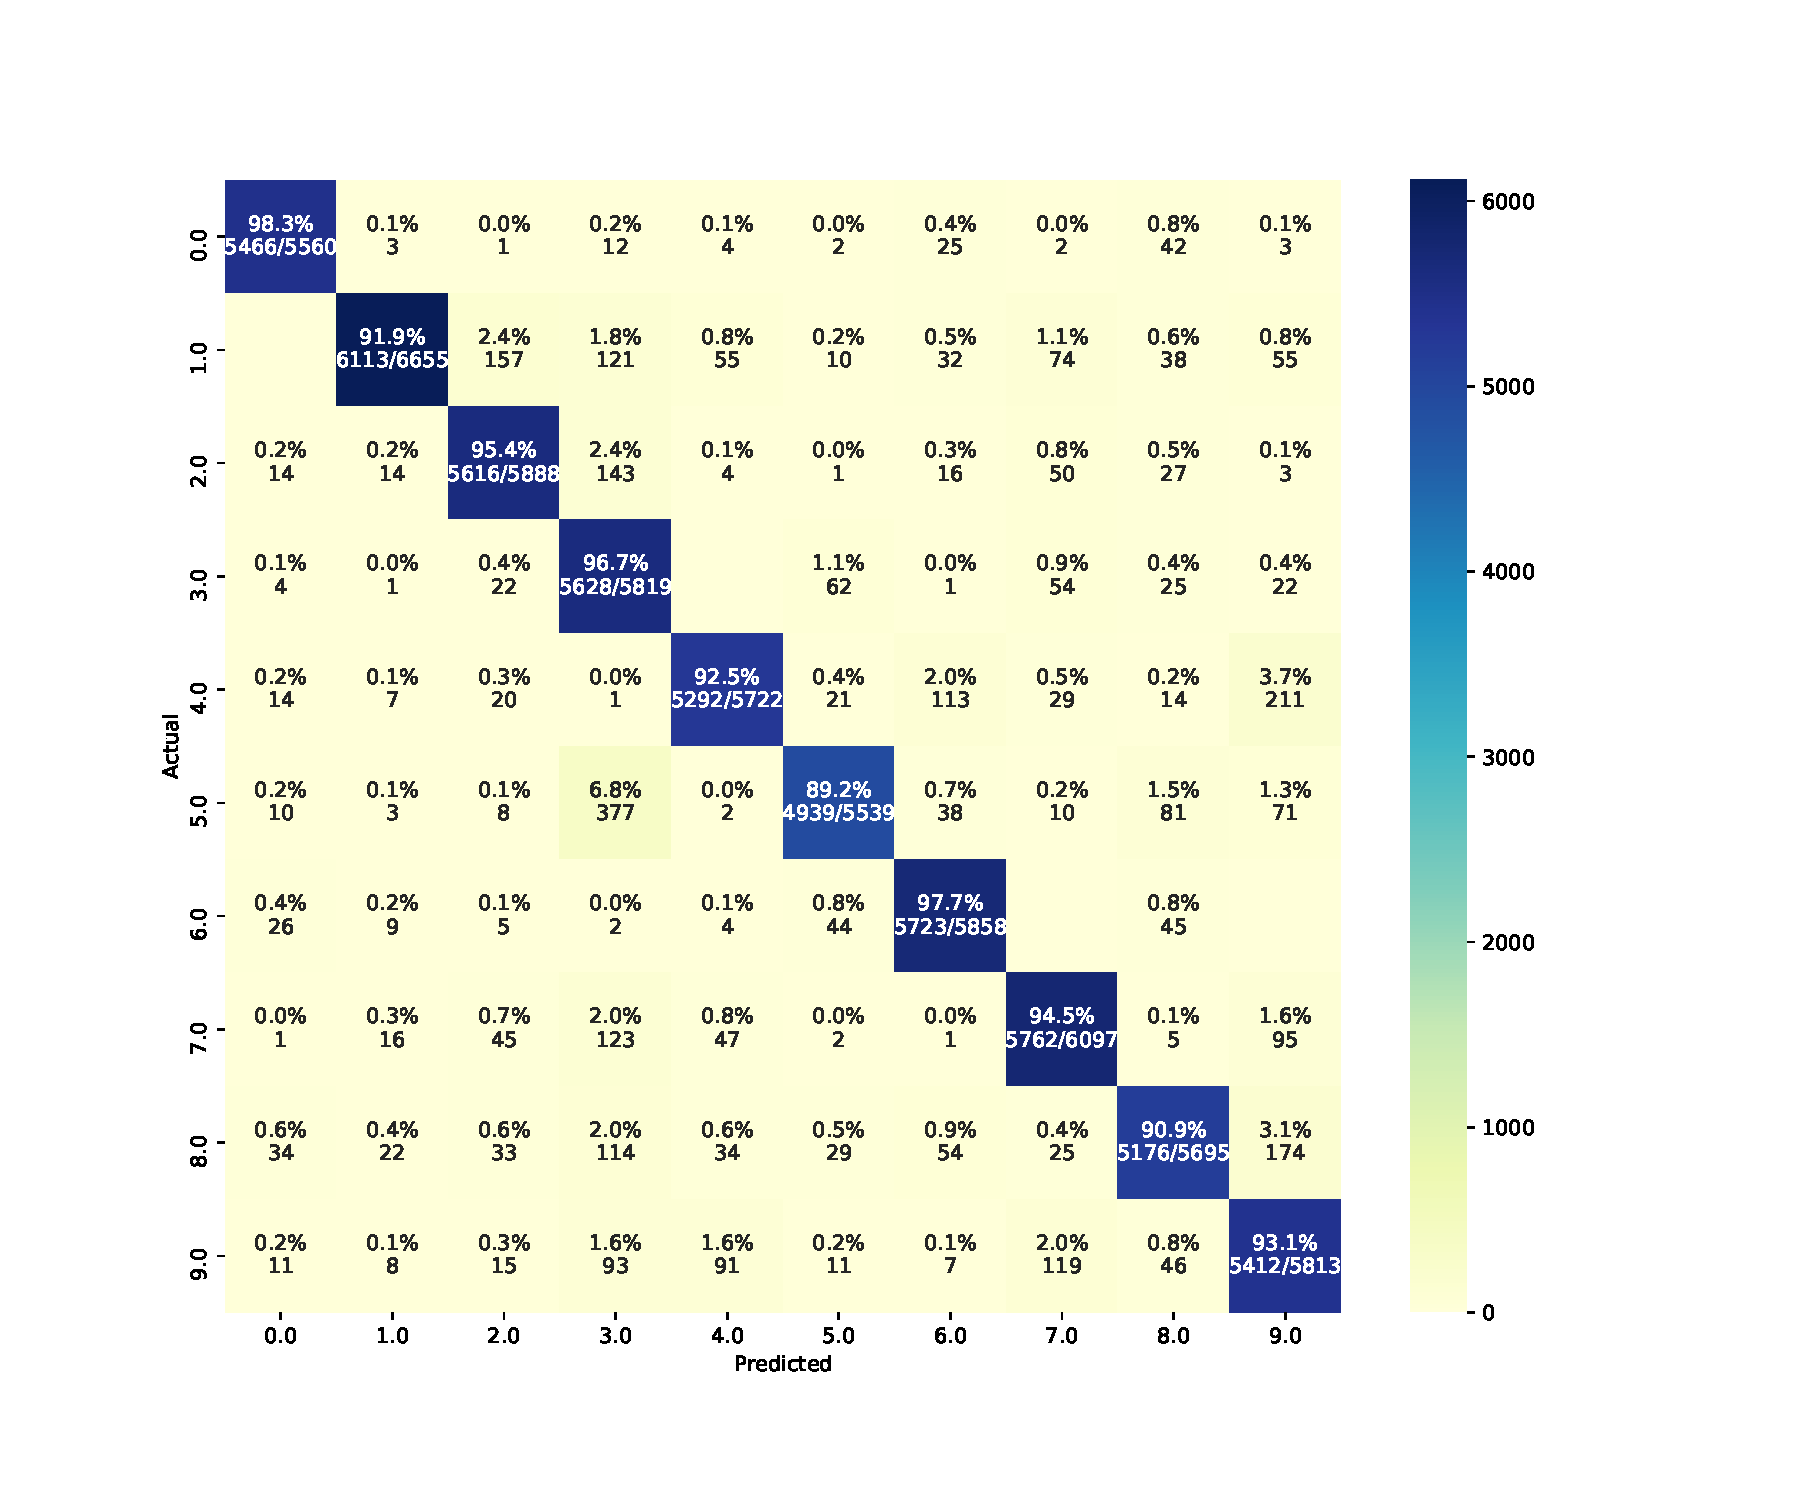
\includegraphics[width=1.1\textwidth]{confusion_knn.pdf}
    \caption{\label{fig:confusion_knn}Matriz de confusão do classificador kNN}
  \end{minipage}\hfill
  \begin{minipage}{.47\textwidth}
    \centering
    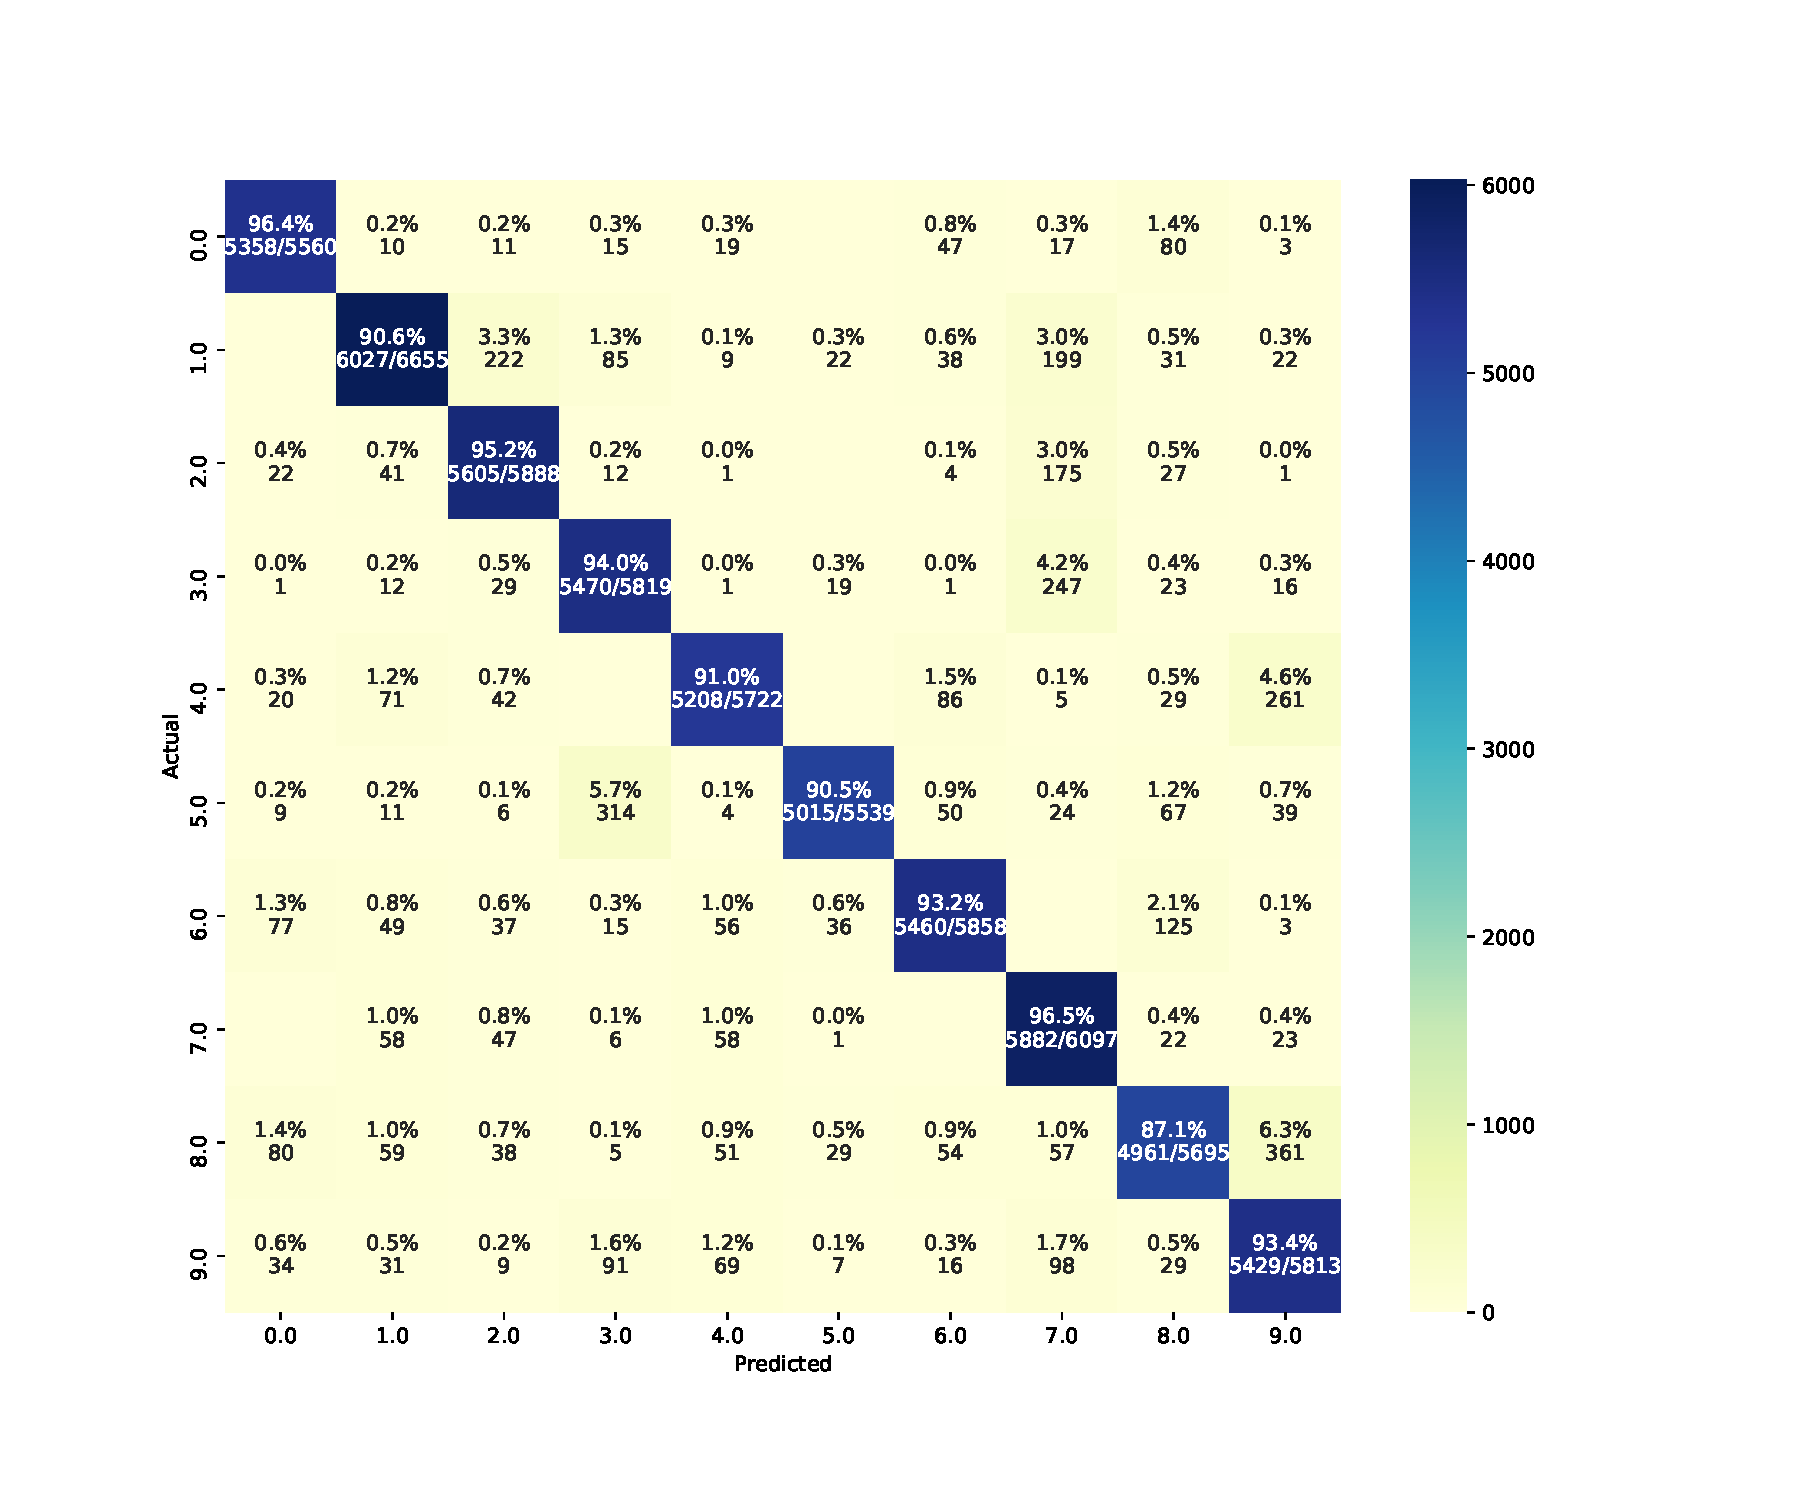
\includegraphics[width=1.1\textwidth]{confusion_lda.pdf}
    \caption{\label{fig:confusion_lda}Matriz de confusão do classificador LDA}
  \end{minipage}
\end{figure}

\begin{figure}[H]
\centering
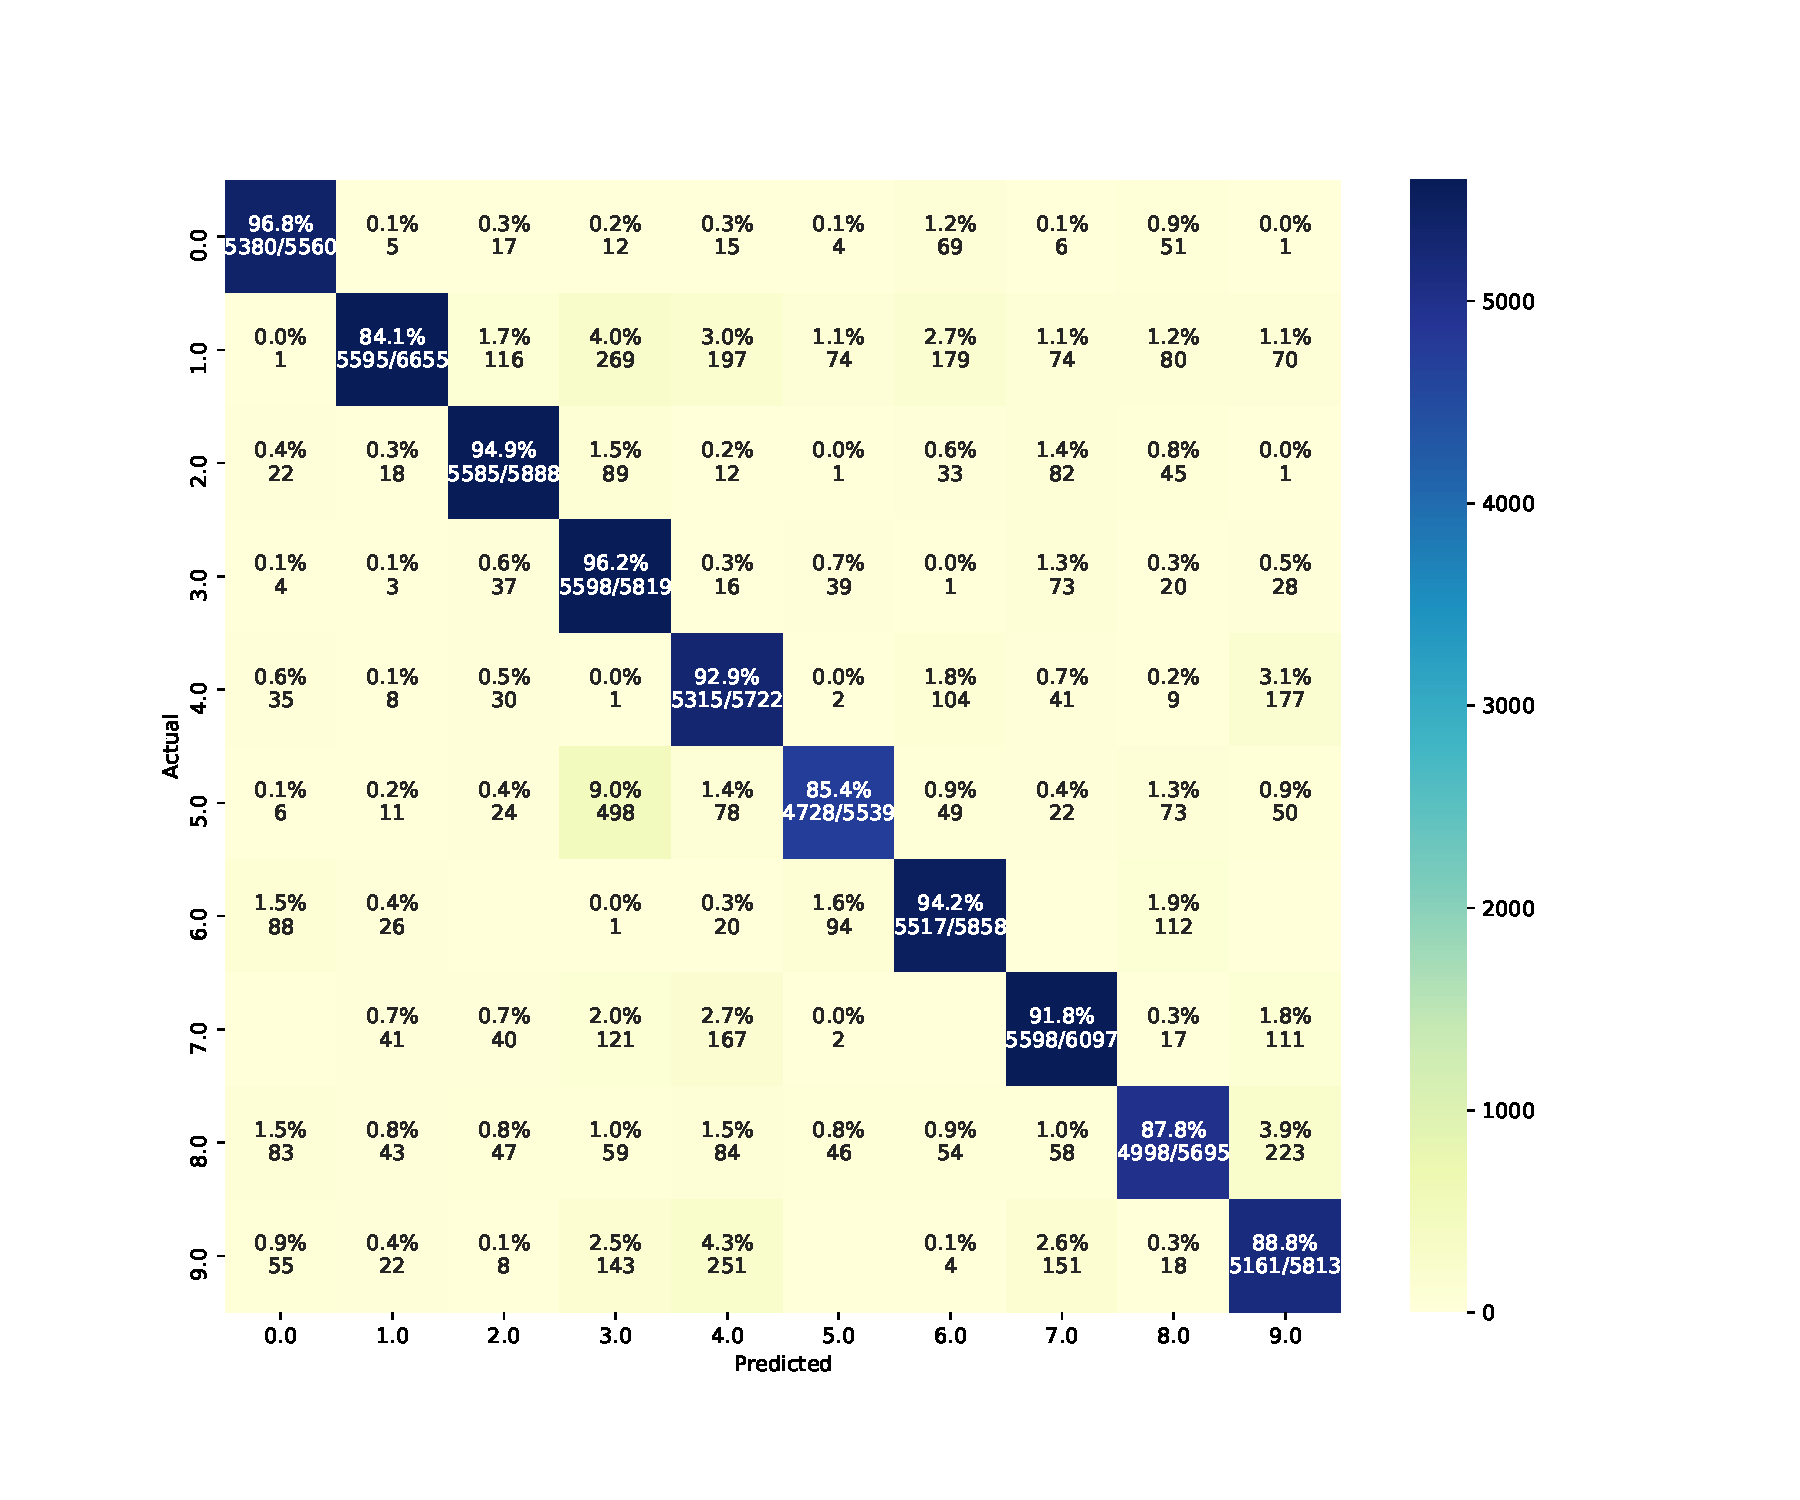
\includegraphics[width=0.8\textwidth]{confusion_logistic.pdf}
\caption{\label{fig:confusion_logistic}Matriz de confusão do classificador Logistic Regression}
\end{figure}

\begin{figure}[H]
\centering
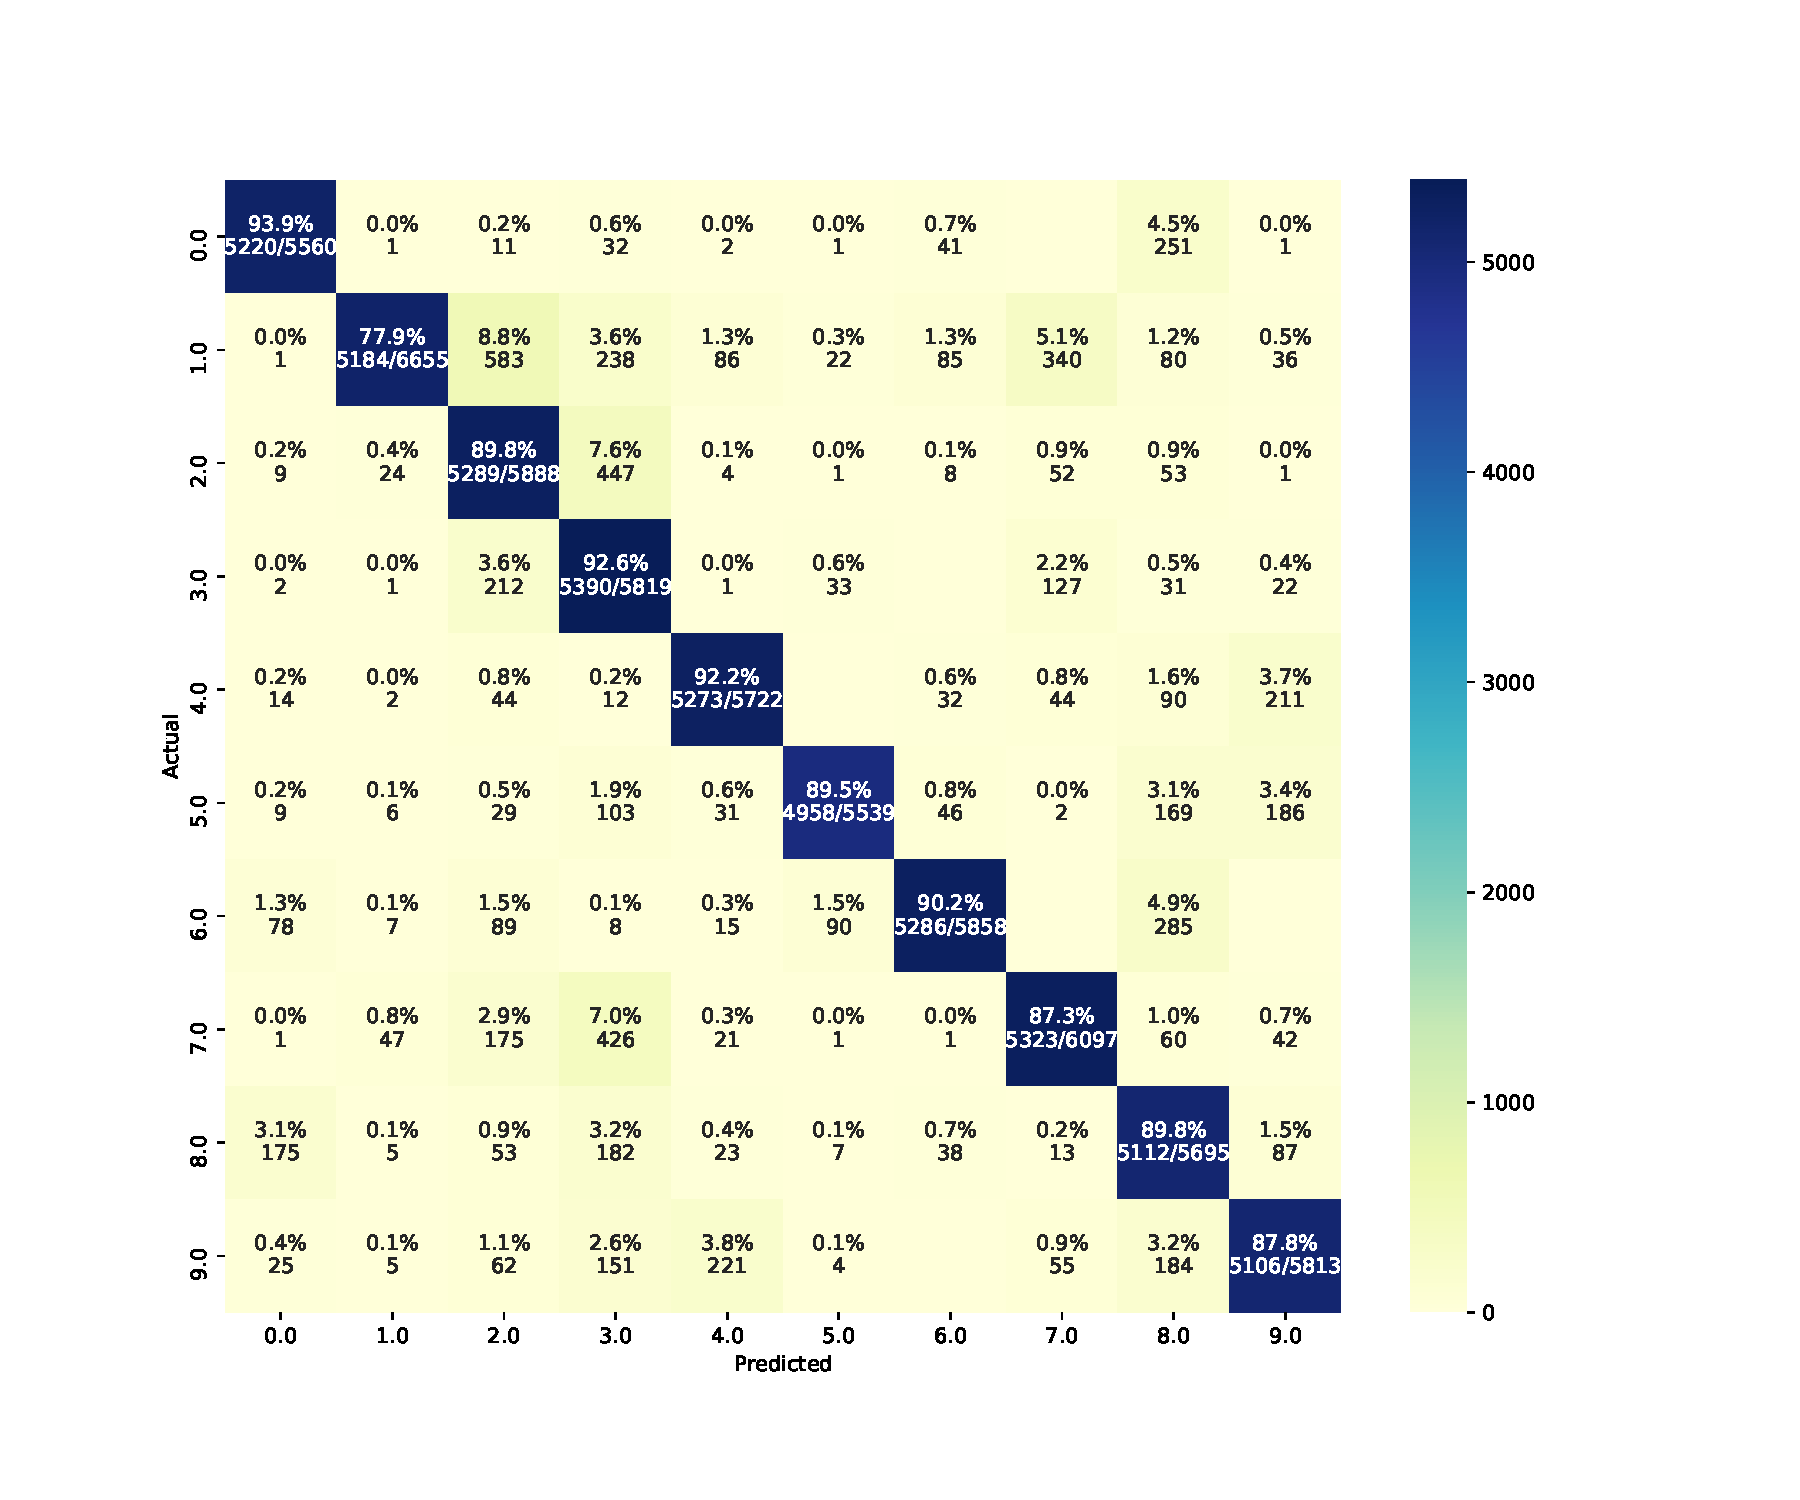
\includegraphics[width=0.8\textwidth]{confusion_naive.pdf}
\caption{\label{fig:confusion_naive}Matriz de confusão do classificador Naive Bayes}
\end{figure}

\begin{figure}[H]
\centering
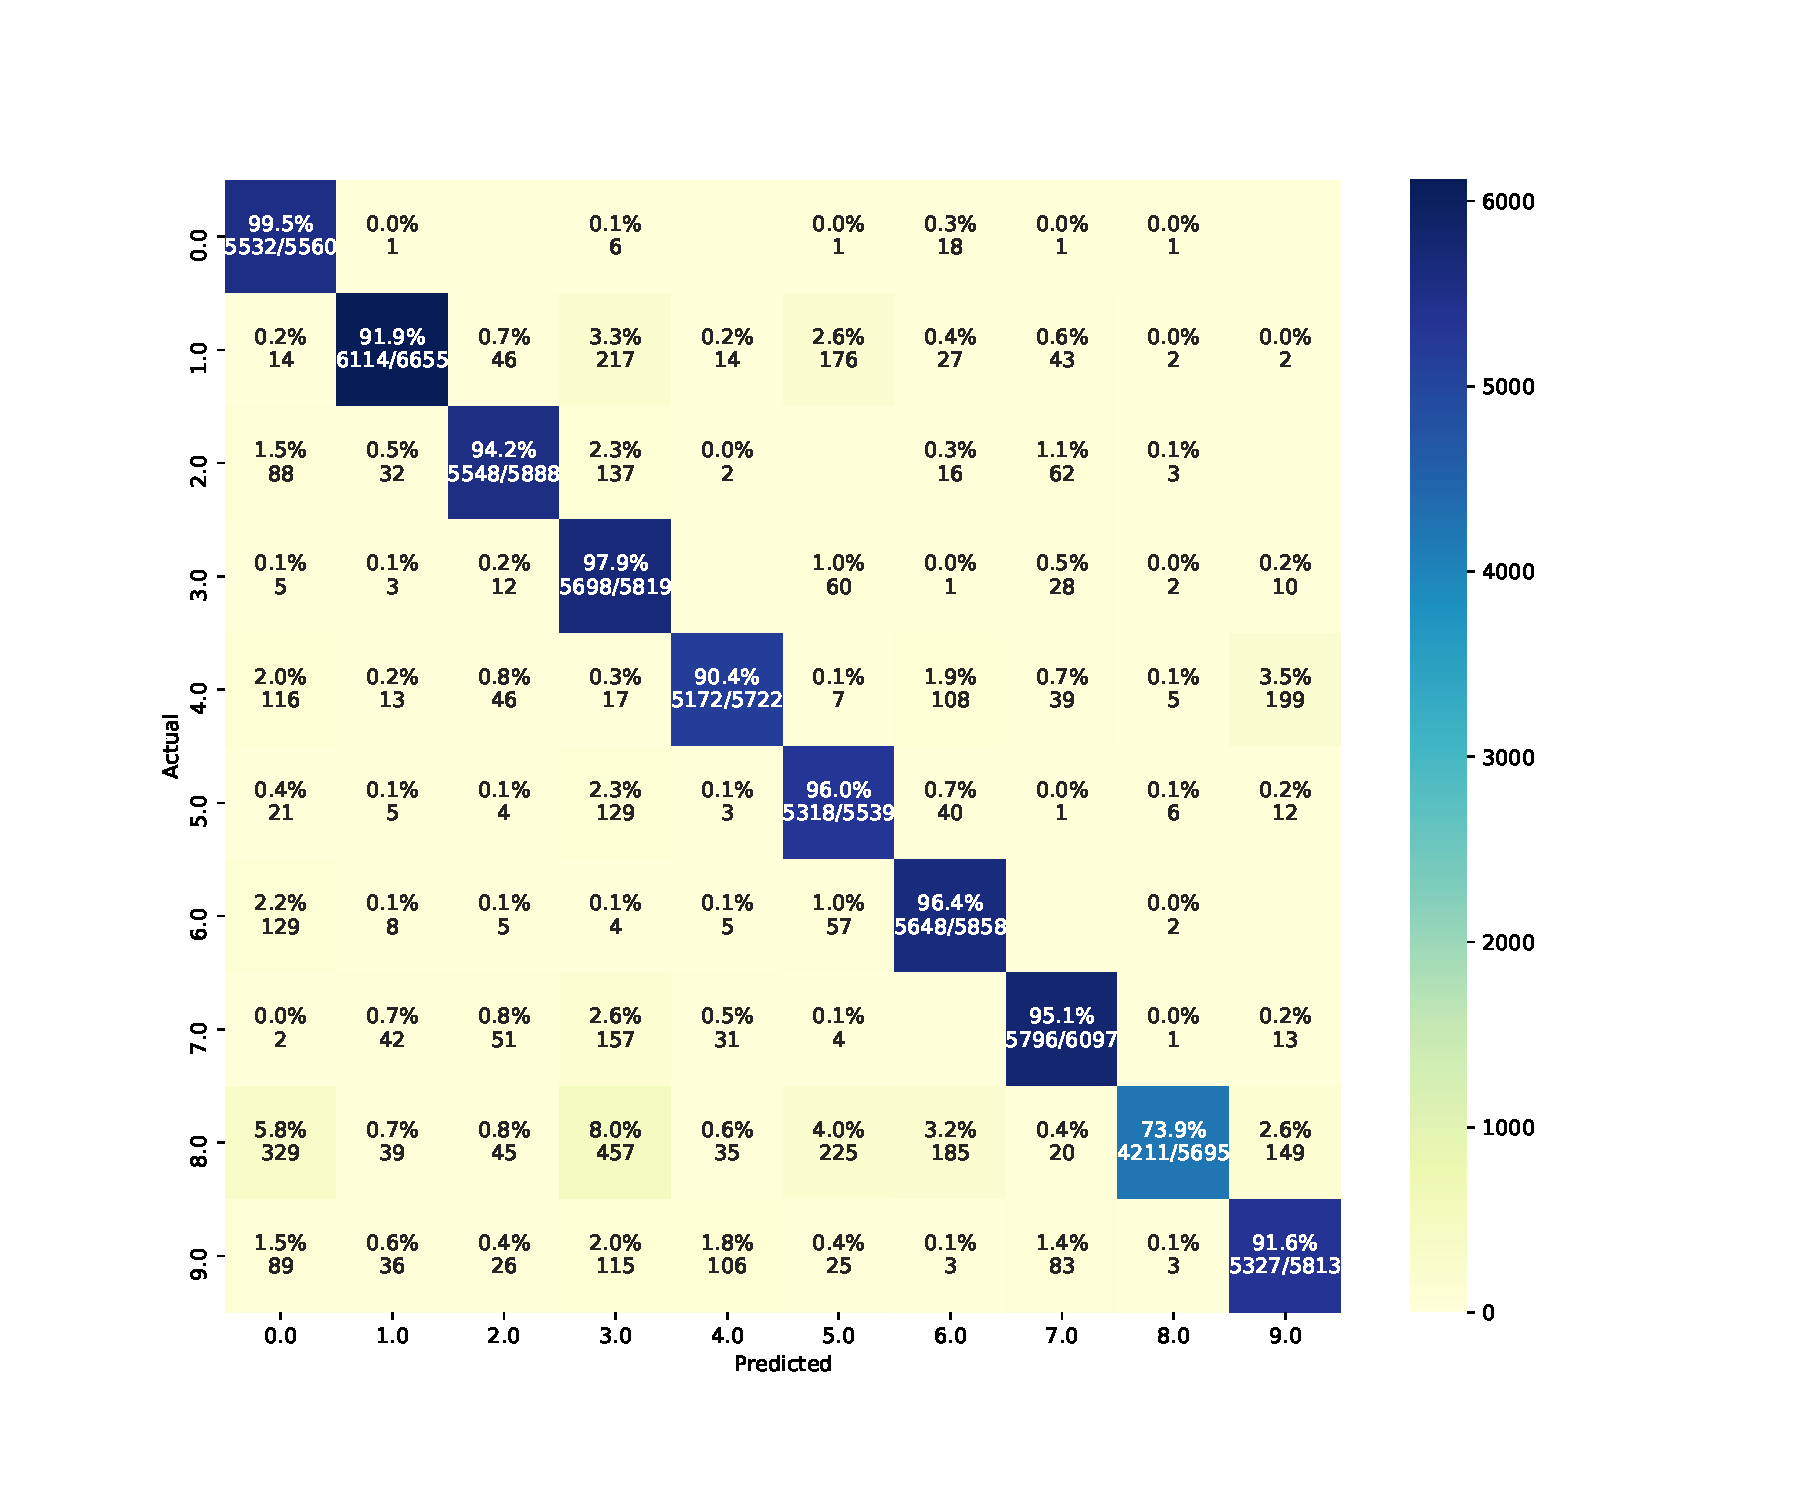
\includegraphics[width=0.8\textwidth]{confusion_perceptron.pdf}
\caption{\label{fig:confusion_perceptron}Matriz de confusão do classificador Perceptron}
\end{figure}

\end{document}

%% Exemplo de figura, copie e cole, substituindo os conteúdos.
\begin{figure}[H]
\centering
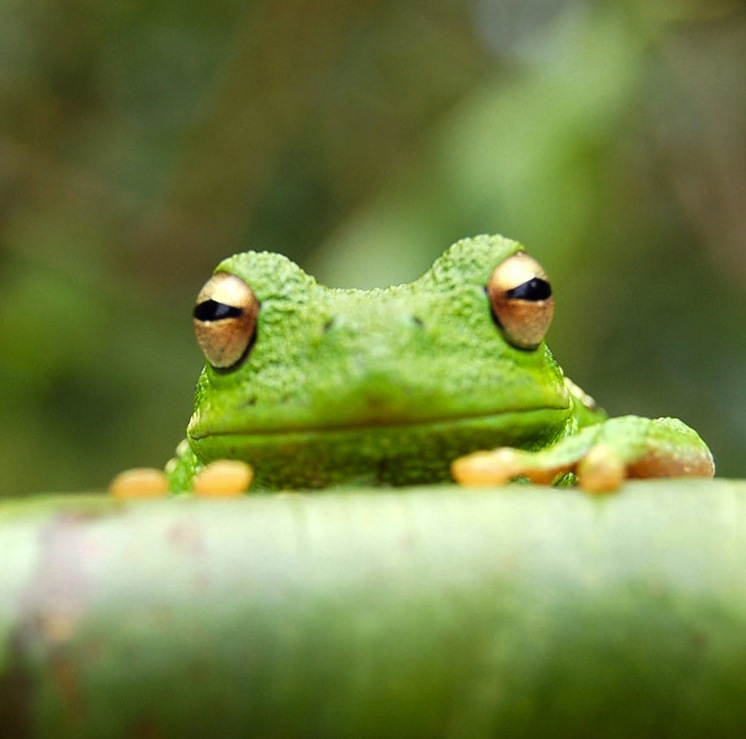
\includegraphics[width=0.3\textwidth]{frog.jpg}
\caption{\label{fig:frog}This frog was uploaded via the project menu.}
\end{figure}

%% Exemplo de tabela, copie e cole, substituindo os conteúdos.
\begin{table}[H]
\centering
\begin{tabular}{l|r}
Item & Quantity \\\hline
Widgets & 42 \\
Gadgets & 13
\end{tabular}
\caption{\label{tab:widgets}An example table.}
\end{table}

\begin{lstlisting}[caption={Relatório do algoritmo kNN},label={relatorio},language=Python]
features_extraction((20,69))
knn("features.txt", 3)
[[ 96   0   0   0   0   1   0   0   0   0]
 [  0  95   0   0   0   0   0   0   0   0]
 [  0   3 103   0   1   0   1   2   1   0]
 [  1   1   0  98   0   1   0   1   1   0]
 [  0   9   2   0  82   0   0   0   0   2]
 [  1   0   0   4   0  91   1   0   0   0]
 [  1   5   0   0   0   0 100   0   0   0]
 [  0   9   0   0   0   0   0  86   0   2]
 [  1   3   0   2   1   1   0   0  79   0]
 [  0   1   0   0   3   0   0   9   1  98]]
              precision    recall  f1-score   support

           0       0.96      0.99      0.97        97
           1       0.75      1.00      0.86        95
           2       0.98      0.93      0.95       111
           3       0.94      0.95      0.95       103
           4       0.94      0.86      0.90        95
           5       0.97      0.94      0.95        97
           6       0.98      0.94      0.96       106
           7       0.88      0.89      0.88        97
           8       0.96      0.91      0.93        87
           9       0.96      0.88      0.92       112

    accuracy                           0.93      1000
   macro avg       0.93      0.93      0.93      1000
weighted avg       0.93      0.93      0.93      1000

0.928
\end{lstlisting}
